% Options for packages loaded elsewhere
\PassOptionsToPackage{unicode}{hyperref}
\PassOptionsToPackage{hyphens}{url}
%
\documentclass[
  man,floatsintext]{apa6}
\usepackage{amsmath,amssymb}
\usepackage{iftex}
\ifPDFTeX
  \usepackage[T1]{fontenc}
  \usepackage[utf8]{inputenc}
  \usepackage{textcomp} % provide euro and other symbols
\else % if luatex or xetex
  \usepackage{unicode-math} % this also loads fontspec
  \defaultfontfeatures{Scale=MatchLowercase}
  \defaultfontfeatures[\rmfamily]{Ligatures=TeX,Scale=1}
\fi
\usepackage{lmodern}
\ifPDFTeX\else
  % xetex/luatex font selection
\fi
% Use upquote if available, for straight quotes in verbatim environments
\IfFileExists{upquote.sty}{\usepackage{upquote}}{}
\IfFileExists{microtype.sty}{% use microtype if available
  \usepackage[]{microtype}
  \UseMicrotypeSet[protrusion]{basicmath} % disable protrusion for tt fonts
}{}
\makeatletter
\@ifundefined{KOMAClassName}{% if non-KOMA class
  \IfFileExists{parskip.sty}{%
    \usepackage{parskip}
  }{% else
    \setlength{\parindent}{0pt}
    \setlength{\parskip}{6pt plus 2pt minus 1pt}}
}{% if KOMA class
  \KOMAoptions{parskip=half}}
\makeatother
\usepackage{xcolor}
\usepackage{graphicx}
\makeatletter
\def\maxwidth{\ifdim\Gin@nat@width>\linewidth\linewidth\else\Gin@nat@width\fi}
\def\maxheight{\ifdim\Gin@nat@height>\textheight\textheight\else\Gin@nat@height\fi}
\makeatother
% Scale images if necessary, so that they will not overflow the page
% margins by default, and it is still possible to overwrite the defaults
% using explicit options in \includegraphics[width, height, ...]{}
\setkeys{Gin}{width=\maxwidth,height=\maxheight,keepaspectratio}
% Set default figure placement to htbp
\makeatletter
\def\fps@figure{htbp}
\makeatother
\setlength{\emergencystretch}{3em} % prevent overfull lines
\providecommand{\tightlist}{%
  \setlength{\itemsep}{0pt}\setlength{\parskip}{0pt}}
\setcounter{secnumdepth}{5}
% Make \paragraph and \subparagraph free-standing
\ifx\paragraph\undefined\else
  \let\oldparagraph\paragraph
  \renewcommand{\paragraph}[1]{\oldparagraph{#1}\mbox{}}
\fi
\ifx\subparagraph\undefined\else
  \let\oldsubparagraph\subparagraph
  \renewcommand{\subparagraph}[1]{\oldsubparagraph{#1}\mbox{}}
\fi
\newlength{\cslhangindent}
\setlength{\cslhangindent}{1.5em}
\newlength{\csllabelwidth}
\setlength{\csllabelwidth}{3em}
\newlength{\cslentryspacingunit} % times entry-spacing
\setlength{\cslentryspacingunit}{\parskip}
\newenvironment{CSLReferences}[2] % #1 hanging-ident, #2 entry spacing
 {% don't indent paragraphs
  \setlength{\parindent}{0pt}
  % turn on hanging indent if param 1 is 1
  \ifodd #1
  \let\oldpar\par
  \def\par{\hangindent=\cslhangindent\oldpar}
  \fi
  % set entry spacing
  \setlength{\parskip}{#2\cslentryspacingunit}
 }%
 {}
\usepackage{calc}
\newcommand{\CSLBlock}[1]{#1\hfill\break}
\newcommand{\CSLLeftMargin}[1]{\parbox[t]{\csllabelwidth}{#1}}
\newcommand{\CSLRightInline}[1]{\parbox[t]{\linewidth - \csllabelwidth}{#1}\break}
\newcommand{\CSLIndent}[1]{\hspace{\cslhangindent}#1}
\ifLuaTeX
\usepackage[bidi=basic]{babel}
\else
\usepackage[bidi=default]{babel}
\fi
\babelprovide[main,import]{english}
% get rid of language-specific shorthands (see #6817):
\let\LanguageShortHands\languageshorthands
\def\languageshorthands#1{}
% Manuscript styling
\usepackage{upgreek}
\captionsetup{font=singlespacing,justification=justified}

% Table formatting
\usepackage{longtable}
\usepackage{lscape}
% \usepackage[counterclockwise]{rotating}   % Landscape page setup for large tables
\usepackage{multirow}		% Table styling
\usepackage{tabularx}		% Control Column width
\usepackage[flushleft]{threeparttable}	% Allows for three part tables with a specified notes section
\usepackage{threeparttablex}            % Lets threeparttable work with longtable

% Create new environments so endfloat can handle them
% \newenvironment{ltable}
%   {\begin{landscape}\centering\begin{threeparttable}}
%   {\end{threeparttable}\end{landscape}}
\newenvironment{lltable}{\begin{landscape}\centering\begin{ThreePartTable}}{\end{ThreePartTable}\end{landscape}}

% Enables adjusting longtable caption width to table width
% Solution found at http://golatex.de/longtable-mit-caption-so-breit-wie-die-tabelle-t15767.html
\makeatletter
\newcommand\LastLTentrywidth{1em}
\newlength\longtablewidth
\setlength{\longtablewidth}{1in}
\newcommand{\getlongtablewidth}{\begingroup \ifcsname LT@\roman{LT@tables}\endcsname \global\longtablewidth=0pt \renewcommand{\LT@entry}[2]{\global\advance\longtablewidth by ##2\relax\gdef\LastLTentrywidth{##2}}\@nameuse{LT@\roman{LT@tables}} \fi \endgroup}

% \setlength{\parindent}{0.5in}
% \setlength{\parskip}{0pt plus 0pt minus 0pt}

% Overwrite redefinition of paragraph and subparagraph by the default LaTeX template
% See https://github.com/crsh/papaja/issues/292
\makeatletter
\renewcommand{\paragraph}{\@startsection{paragraph}{4}{\parindent}%
  {0\baselineskip \@plus 0.2ex \@minus 0.2ex}%
  {-1em}%
  {\normalfont\normalsize\bfseries\itshape\typesectitle}}

\renewcommand{\subparagraph}[1]{\@startsection{subparagraph}{5}{1em}%
  {0\baselineskip \@plus 0.2ex \@minus 0.2ex}%
  {-\z@\relax}%
  {\normalfont\normalsize\itshape\hspace{\parindent}{#1}\textit{\addperi}}{\relax}}
\makeatother

\makeatletter
\usepackage{etoolbox}
\patchcmd{\maketitle}
  {\section{\normalfont\normalsize\abstractname}}
  {\section*{\normalfont\normalsize\abstractname}}
  {}{\typeout{Failed to patch abstract.}}
\patchcmd{\maketitle}
  {\section{\protect\normalfont{\@title}}}
  {\section*{\protect\normalfont{\@title}}}
  {}{\typeout{Failed to patch title.}}
\makeatother

\usepackage{xpatch}
\makeatletter
\xapptocmd\appendix
  {\xapptocmd\section
    {\addcontentsline{toc}{section}{\appendixname\ifoneappendix\else~\theappendix\fi\\: #1}}
    {}{\InnerPatchFailed}%
  }
{}{\PatchFailed}
\keywords{Psycholinguistics, holistic storage, language processing, lexical processing, phonological processing}
\usepackage{csquotes}
\usepackage[section]{placeins}
\ifLuaTeX
  \usepackage{selnolig}  % disable illegal ligatures
\fi
\IfFileExists{bookmark.sty}{\usepackage{bookmark}}{\usepackage{hyperref}}
\IfFileExists{xurl.sty}{\usepackage{xurl}}{} % add URL line breaks if available
\urlstyle{same}
\hypersetup{
  pdftitle={The effects of frequency and predictability on the recognition of up in English multi-word phrases.},
  pdfauthor={Zachary Houghton1, Jungah Lee2, Casey Felton1, Georgia Zellou1, \& Emily Morgan1},
  pdflang={en-EN},
  pdfkeywords={Psycholinguistics, holistic storage, language processing, lexical processing, phonological processing},
  hidelinks,
  pdfcreator={LaTeX via pandoc}}

\title{The effects of frequency and predictability on the recognition of \emph{up} in English multi-word phrases.}
\author{Zachary Houghton\textsuperscript{1}, Jungah Lee\textsuperscript{2}, Casey Felton\textsuperscript{1}, Georgia Zellou\textsuperscript{1}, \& Emily Morgan\textsuperscript{1}}
\date{}


\shorttitle{Effects of frequency and predictability on the recognition of \emph{up}.}

\authornote{

Correspondence concerning this article should be addressed to Zachary Houghton, . E-mail: \href{mailto:znhoughton@ucdavis.edu}{\nolinkurl{znhoughton@ucdavis.edu}}

}

\affiliation{\vspace{0.5cm}\textsuperscript{1} University of California, Davis\\\textsuperscript{2} Chosun University}

\abstract{%
The question of what is stored is one that has drawn a lot of attention in the last few decades, and while the general consensus is that a lot more is stored than we previously realized, it is still largely unclear what factors drive storage. For example, some have argued that frequency drives storage, while others have posited that predictability drives storage. Further, it is what the processing consequences of storage are. For example, it is possible that stored items fuse together, losing some amount of their internal structure. The present paper examines both of these questions by looking at the recognizability of the segment \emph{up} in English V+\emph{up} phrases. We find that recognition follows a u-shaped pattern for both frequency and predictability suggesting that stored items may lose some amount of their internal representation.
}



\begin{document}
\maketitle

\hypertarget{introduction}{%
\section{Introduction}\label{introduction}}

The question of to what extent language processing involves processing individual pieces of the utterance versus accessing stored representations from memory is one that has gained a lot of attention in the Psycholinguistics literature in the last few decades (e.g., Bybee, 2002, 2003; Goldberg, 2003; Nooteboom, Nooteboom, Weerman, \& Wijnen, 2002; Stemberger \& MacWhinney, 1986, 2004). For example, take the classic Halloween greeting, \emph{trick or treat}. When you hear the phrase trick or treat do you process it compositionally, processing each word in the utterance and then combining them into a single parse? Or do you access a single stored representation from memory?,

The literature has traditionally assumed the former, arguing that processing is almost completely compositional: each piece is accessed individually and then combined to form the larger meaning, reserving some exceptions for idioms and other outliers. These theories gained popularity partially because storage was thought to be a valuable resource that was taken up only by units that necessitated storage (see Nooteboom et al., 2002 for a further discussion on the traditional assumptions of storage), perhaps due to the limited storage space of sophisticated computers at the time. In recent times, however, we've learned that the brain may have dramatically more space for storage than we had previously realized, with an upper bound of 108432 bits (Wang, Liu, \& Wang, 2003). This is magnitudes larger than any current estimate of how much storage language requires (Indeed, Mollica \& Piantadosi, 2019 estimated that, in terms of linguistic information, humans store only somewhere between one million and ten million bits of information, meaning that even their upper estimate is well within the capacity of the brain).

On the other hand, usage-based theories posit that some complex phrases may be accessed holistically from memory, and whether it is accessed as a single chunk is driven by the distribution of the input language. For example, rather than being purely determined by the degree of compositionality of an utterance, usage-based theories suggest that other factors, such as how frequent the phrase is, may also play a role. According to these theories, frequency of use may lead to compositional items, e.g., multi-word phrases, being stored as a holistic unit which can be accessed from memory (Arnon \& Snider, 2010; Hay, 2001; e.g., Kapatsinski, 2018; Kapatsinski \& Radicke, 2009; Lee \& Kapatsinski, 2015; Morgan \& Levy, 2016; Stemberger \& MacWhinney, 1986, 2004; Tomasello, 2005).

While it has become a dominant view in the field that at least some multi-word items are stored, it remains unclear, however, what exactly the size of the units being stored is and, more so, what the factors driving storage are. Further, if larger-than-word representations are being stored, what are the consequences of this on language processing?

\hypertarget{evidence-of-holistic-storage}{%
\subsection{Evidence of Holistic Storage}\label{evidence-of-holistic-storage}}

Usage-based theories owe at least part of their rise in popularity to the accumulation of evidence for holistic multi-word storage (e.g., Bybee \& Scheibman, 1999; Christiansen \& Arnon, 2017; Hay, 2001; Stemberger \& MacWhinney, 1986, 2004; Zwitserlood, 2018), an abundance of which comes from the phonology literature. For example, Bybee and Scheibman (1999) demonstrated that the word \emph{don't} is both more reduced and reduced to a larger extent in the phrase \emph{I don't know} (which can be reduced to just a nasal syllable that maintains the intonation of the original phrase!) than in other words containing \emph{don't}. In other words, the phrase \emph{I don't know} seems to have its own mental representation (since if it was the case that the representation of \emph{I don't know} and \emph{don't} were the same, then one would expect \emph{don't} to be equally reduced in both cases). Additionally, in Korean, tensification often occurs after the future marker \emph{-l}, and the rate of this tensification is higher for high-frequency phrases than low-frequency phrases, further suggesting that high-frequency phrases may be stored holistically (Yi, 2002).

In addition to phonological effects , the Psycholinguistics literature has also provided an abundance of evidence for multi-word storage. For example, Siyanova-Chanturia, Conklin, and Heuven (2011) demonstrated that binomial phrases (e.g., \emph{cat and dog}) are read faster in their more frequent ordering than in their less frequent ordering. Specifically, participants read sentences containing binomial phrases (e.g., \emph{bread and butter}) in both their more frequent and less frequent orderings (e.g., \emph{bread and butter} vs \emph{butter and bread}). They found that both native and non-native speakers read the phrase faster in its more frequent ordering than in its less frequent ordering, suggesting that frequent binomial phrases are stored holistically. Further, in a follow-up study, Morgan and Levy (2016) demonstrated that these ordering preferences for frequent binomials are not due to abstract ordering preferences (e.g., a preference for short words before long words), providing additional evidence that frequent binomials are stored holistically.

Further, there is also evidence of multi-word storage from the learning literature. For example, Siegelman and Arnon (2015) demonstrated that learning is facilitated by attending to the whole utterance, as opposed to attending to each individual word. Specifically, they used an artificial language paradigm to examine adult L2 learners' ability to learn grammatical gender. They found that adults learn much better when they are presented with unsegmented utterances rather than segmented utterances. Indeed, even sophisticated language learning models owe at least part of their modern day success in focusing on sentence-level representations rather than individual word-level representations\footnote{One of the biggest advancements in large language models has been the transition from Long Short-Term Memory models (LSTMs) to Transformer models. A key difference between these models is that LSTMs take as their input a word and predict as their output an upcoming word (Hochreiter \& Schmidhuber, 1997). In contrast, Transformer models take as their input an entire sentence and predict as their output an individual word (citation). In this way, it seems both humans and language models may benefit from focusing on the utterance, rather than individual words. Although it is important to note that this is by no means the only difference between these models (Vaswani et al., 2017).}.

\hypertarget{what-drives-storage}{%
\subsection{What Drives Storage?}\label{what-drives-storage}}

Despite the evidence of multi-word holistic storage, however, it is still largely unclear what factors drive storage. Indeed, humans seem to be sensitive to all kinds of statistical information, including both frequency\footnote{Frequency can be further broken down into token and type frequency, so treating frequency as a singular category is a bit of a simplification.} (Bybee \& Scheibman, 1999; Kapatsinski \& Radicke, 2009; Lee \& Kapatsinski, 2015; e.g., Maye \& Gerken, 2000) and predictability (e.g, Olejarczuk, Kapatsinski, \& Baayen, 2018; Ramscar, Dye, \& Klein, 2013).

Traditionally, frequency has been assumed to be the driving factor behind multi-word storage, and for good reason. Indeed, most of the examples of storage given so far have been with respect to frequency. Perhaps the most famous series of studies demonstrating this were conducted by Bybee (Bybee, 2003; Bybee \& Hopper, 2001; Bybee \& Scheibman, 1999). In a series of studies, Bybee and colleagues demonstrated that a variety of words are reduced more in high-frequency contexts than low-frequency context (additionally see Kapatsinski, 2021 for further discussion of this). For example, in addition to the earlier examples, \emph{going to} can be reduced in the frequent future marker, \emph{gonna}, but not in the less frequent verb phrase construction describing motion (e.g., *\emph{gonna the store}, Bybee, 2003). This mirrors patterns we see on a word-level (which for the most part must be stored in any theory of processing). For example, the reduction of vowels to schwa in English is more advanced in high-frequency words than low-frequency words (Bybee, 2003; Hooper, 1976). In other words, the fact that sound changes occur differently depending on the frequency of the word suggests that they have separate representations (i.e., holistic storage).

On the other hand, predictability has also been shown to play a crucial role in learning (Olejarczuk et al., 2018; Ramscar et al., 2013; Saffran, Aslin, \& Newport, 1996). For example, Olejarczuk et al. (2018) demonstrated that when learning new phonetic categories, learners don't just pay attention to co-occurrence rates, but actively try to predict upcoming events, suggesting that the learning of phonetic categories is also driven by prediction. Further, in learning new words, Ramscar et al. (2013) demonstrated that children are sensitive to how predictable a cue is of an outcome (e.g., a high-frequency cue will be ignored if it isn't predictive of a specific outcome). Indeed, even arguably the most popular statistical learning paper demonstrates the importance of predictability in learning (Saffran et al., 1996). In their classic paper, Saffran et al. (1996) demonstrated that children keep track of transitional probabilities -- a measurement of predictability -- to segment the speech stream. While it is of course important to note that none of these are evidence that predictability drives multi-word storage, the connection may be clear by now: the units that we learn may likely be the units we store. If predictability drives what we learn, it may also drive what we store. That is, if high-predictability words are learned together, they may be stored together. Thus given the abundance of evidence for both frequency and predictability effects in language, it remains unclear which of these factors drives storage. Indeed, it may be possible that a combination of both drives multi-word storage.

\hypertarget{processing-consequences-of-storage}{%
\subsection{Processing Consequences of Storage}\label{processing-consequences-of-storage}}

The previous section demonstrated the abundance of evidence that a lot more than just monomorphemic words and idioms are stored, and given that, one more important question to consider is what exactly the processing consequences of storage are. Specifically, do the stored units maintain their own internal representation (or did they ever even have it to begin with)?

Indeed, there seems to be some evidence that multi-word phrases may lose (or perhaps never had) some amount of their internal structure. For example, Kapatsinski and Radicke (2009) demonstrated that in high frequency V+\emph{up} constructions, it is harder to recognize the segment \emph{up} (with respect to medium-frequency V+\emph{up} constructions), suggesting that these items may have a holistic representation. Participants were given different auditory sentences and were tasked with pressing a button if they heard the segment up. Interestingly, they found that recognizability of \emph{up} follows a U-Shaped pattern. That is, participants had trouble recognizing the parts of low frequency phrasal verbs, but for higher frequency phrasal verbs they were better at recognizing the parts, until reaching the highest frequency words, where they were slower Kapatsinski \& Radicke (2009). Though it's important to note that they do not take into account predictability. A visualization of what a stored representation with and without internal structure may look like is presented in Figure \ref{fig:lossInternal}. The left tree represents the phrase \emph{pick up} stored with its internal structure still intact, whereas the right tree represents \emph{pick up} stored without internal structure.



\begin{figure}

{\centering 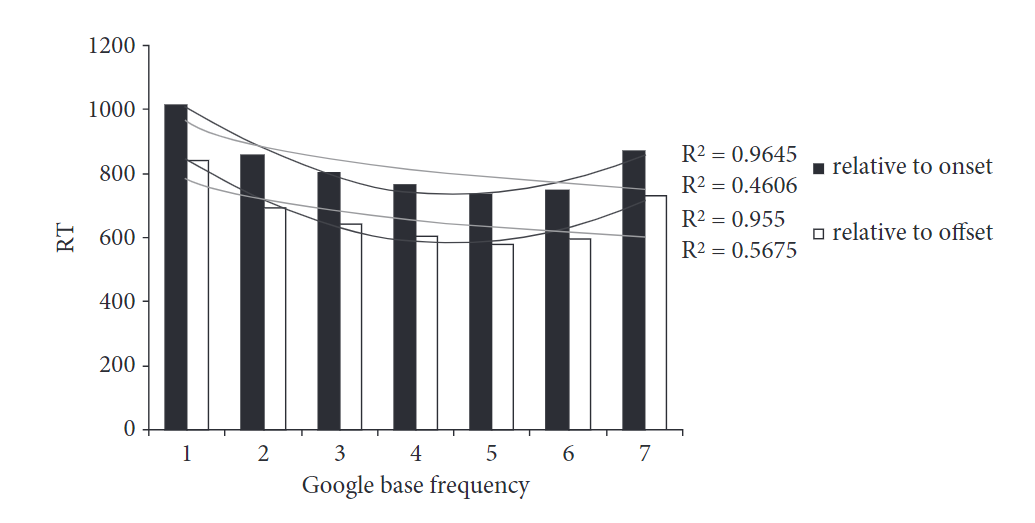
\includegraphics[width=0.7\linewidth]{Figures/kapatsinskiradicke_graph} 

}

\caption{The U-shaped effect of the frequency of verb+\emph{up} constructions on the speed with which up is detected, reproduced from Kapatsinski and Radicke (2009).}\label{fig:kapatsinskiplot}
\end{figure}



\begin{figure}

{\centering 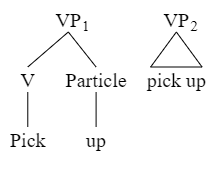
\includegraphics[width=0.3\linewidth]{Figures/syntax_tree} 

}

\caption{A diagram of two ways the word \emph{pick up} could be stored. The left tree demonstrates a stored representation of \emph{pick up}, where the internal structure is still intact. The right tree demonstrates a holistically stored unit, where there is a loss of internal structure. Note that these are stored structures, as opposed to a compositional representation of \emph{pick up} which would be comprised of the individual representations \emph{pick} and \emph{up}.}\label{fig:lossInternal}
\end{figure}

Additionally, there is evidence of processing consequences of storage from the word-recognition literature, where it has been found that it is harder to recognize letters in high-frequency words (Healy, 1976, 1994; Minkoff \& Raney, 2000). For example, Healy (1976) examined participants' ability to recognize letters in various words. He found that people were worse at recognizing the letter \emph{t} in \emph{the} than in other lower frequency words, which suggests that even words can develop a representation that seems to lack internal structure. If it is the case that \emph{the} is recognized as a composition of its parts, then it's unclear what would explain these results (c.f., Kapatsinski \& Radicke, 2009, who suggested that one explanation is that people don't fixate as long on high-frequency and function words, of which \emph{the} is both).

\hypertarget{present-study}{%
\subsection{Present Study}\label{present-study}}

The present study examines the factors that drive storage and the processing consequences of storage by extending Kapatsinski and Radicke (2009) to look at the effects of both frequency, predictability, and their interaction on the processing of phrasal verbs. Similar to Kapatsinski and Radicke (2009), participants are tasked with pressing a button once they hear the segment up (which in our study occurs in either phrasal verbs as a particle or words), but in our case the stimuli varied in both frequency and predictability. Since frequency effects are rather robust in the literature, we should at the very least see a negative correlation between frequency and reaction time (up to perhaps a certain point, where recognition may get harder, i.e an increase in reaction time). The effects of predictability on recognition times, however, are still relatively untested in the literature. If predictability is not a driving factor of storage, we should see only frequency effects on the recognizability of \emph{up}. Further, if storage does result in a loss of internal structure, we should see similar effects to those found in Kapatsinski and Radicke (2009). Specifically, we should see some sort of u-shaped effect, where recognition gets easier until we get to the stored units, where recognizability should then become harder.

\hypertarget{methods}{%
\section{Methods}\label{methods}}

\hypertarget{participants}{%
\subsection{Participants}\label{participants}}

Participants were recruited through the University of California Linguistics/Psychology Human Subjects Pool. 350 people participated in this study and were compensated in the form of SONA credit. All participants self-reported being native English speakers. Additionally, 44 participants were excluded due to an accuracy score below our threshold of 70\%, leaving a total of 306 participants for the data analysis.

\hypertarget{materials}{%
\subsection{Materials}\label{materials}}

We searched the Google n-grams corpus for the most predictable and the highest frequency phrases that matched our criteria of containing a Verb immediately followed by the word \emph{up}. We operationalized predictability as the ratio of the probability of \emph{up} occurring immediately after the verb to the probability of any other word occurring (Equation \eqref{eq:logOdds}:

\begin{equation}
\label{eq:logOdds}
\frac{\mathrm{count(\textit{Verb+up})}}{\mathrm{count(\textit{Verb})} - \mathrm{count(\textit{Verb+up})}} 
\end{equation}

In non-mathematical terms, the above equation quantifies how likely up is to follow after the verb relative to every other word that could follow. For example, the odds ratio of \emph{pick up} would be the number of times the entire verb phrase occurs -- \emph{pick up} -- divided by the number of times the verb -- \emph{pick} -- occurs without up following it.

For the purposes of the present study, we aimed to gather a variety of phrases that varied in both their predictability and frequency and their combination. In order to do this, we extracted the 50 most frequent Verb+\emph{up} items and the 50 most predictable ones. Next, we selected 100 more by randomly sampling from the remaining items. In order to ensure stable predictability estimates we eliminated words that a college-aged speaker wouldn't have heard more than 10 times.\footnote{Levy, Fedorenko, Breen, and Gibson (2012) extrapolated that the average college-aged speaker has heard about 350 million words in their lifetime. Thus we excluded items that had a frequency smaller than 10 per 350 million.} We then visually inspected the data to confirm that our data spanned across both the frequency and predictability continuum. This distribution is presented in Figure \ref{fig:stimplot2} below:

\begin{figure}

{\centering 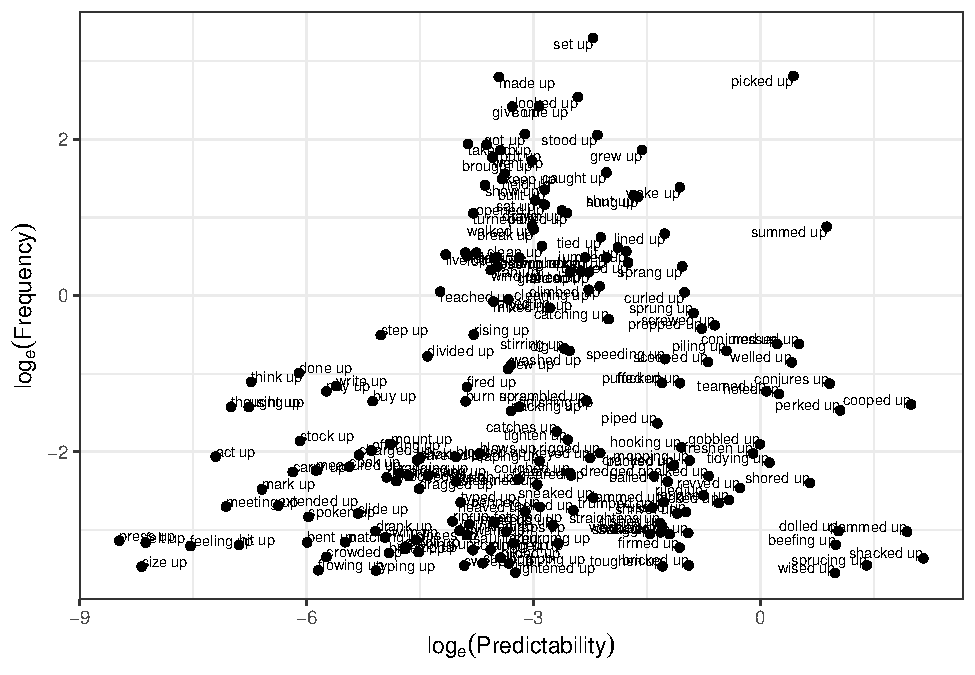
\includegraphics[width=0.8\linewidth]{write-up_files/figure-latex/stimplot2-1} 

}

\caption{log-predictability by log-frequency (per million) plot of our items.}\label{fig:stimplot2}
\end{figure}

We also searched the same corpus for words that contained the segment \emph{up} (e.g., \emph{cupcake}). In order to gather a subset of words that roughly match the frequency range of our experimental stimuli, we extracted the 50 most frequent words, then sampled from the rest of the dataset to gather an additional 100 words. These 350 items together comprise our stimuli.

Finally, we also coded our stimuli for whether they were phrasal verbs or not. This coding was done based on whether they could syntactically alternate between having the noun within the phrase and having the noun after the phrase. For example, since both \emph{pick the cat up} and \emph{pick up the cat} are grammatical, \emph{pick up} was classified as a phrasal verb. Each item was checked by two of the authors. Disagreement was easily resolved by discussion and an agreement was reached for every item.

For each item, we constructed two sentences: one sentence which contained \emph{up}, and one sentence that was identical except that it didn't include the segment \emph{up} for a total of 700 experimental items.

In summary, our stimuli were comprised of 200 Verb+\emph{up} phrases that varied in both frequency and predictability, 150 words that contained \emph{up}, and 350 filler sentences which were matched with our experimental sentences with the exception of having \emph{up} replaced with a different morpheme or word.

After creating the sentences, a Native English speaker then recorded each sentence in a random order to minimize any list effect. We subsequently equalized the amplitude such that every sentence was roughly the same loudness.

\hypertarget{procedure}{%
\subsection{Procedure}\label{procedure}}

Participants were presented with audio sentences via Pavlovia (\url{https://pavlovia.org/}) a website for presenting PsychoPy experiments. Each participant was presented with 3 practice trials and then 350 sentences. While we had a total of 700 sentences, participants didn't see both the filler and experimental sentence for the same item, thus they only saw half of the stimuli. The order of the sentences was random and exactly half of the sentences contained the target segment (to avoid biasing the participants towards a specific response). Participants were instructed to press a key as soon as they heard the segment up, or to press a separate key at the end of the sentence if they did not hear the segment in the sentence. We then recorded their reaction time of the button press. The experiment took approximately 40 minutes.

\hypertarget{analysis}{%
\subsection{Analysis}\label{analysis}}

The data\footnote{The stimuli, data, and analyses scripts can all be found freely available here: \url{https://github.com/znhoughton/Recognizability-Experiment}} was analyzed using General Additive Mixed models, as implemented in the \emph{mgcv} package (Wood, 2011) within the R programming environment (R Core Team, 2023). General Additive Mixed Models are models that allow us to model our outcome variable as a combination of the predictors. GAMMs differ from generalized linear regression models in that they allow the predictors to be modeled as non-linear functions, similar to polynomial regression. Specifically, in a Generalized Additive Mixed Model, beta-coefficients are replaced with a smooth function, which is a combination of splines. The more splines that we include, the more wiggly our line will be. In order to avoid overfitting, GAMMs also include a penalty term, \(\lambda\), which can be modified to penalize more wiggly lines that aren't justified by the data. While the predictors are allowed to vary non-linearly, the linking function in our case was linear (i.e., response time varied linearly with the spline functions).

For all of our models, the dependent variable was the time it took for participants to react to the onset of the target segment (i.e., the time it took participants to react to the word after hearing it). For the first model, the predictors were the interaction between log-predictability and log-frequency, which was allowed to vary non-linearly, and duration of the segment, which was not allowed to vary non-linearly. Additionally, we also included random intercepts for participant, trial, and item, as well as random slopes for predictability by participants, frequency by participant, and trial by participant. Our model formula is included below in Equation \eqref{eq:gammInteraction}:

\begin{equation}
\begin{aligned}
\label{eq:gammInteraction}
log(RT) & \sim ti(Predictability, Frequency) + Duration + s(participant, bs = `re\text{'}) + s(Item, bs = `re\text{'}) \\
& + s(trial, bs = `re\text{'}) + s(Predictability, Frequency, participant, bs = `re\text{'}) 
\end{aligned}
\end{equation}

We also ran an additional analysis similar to the first model, but allowing the interaction to vary for Phrasal vs non-phrasal verbs. Specifically, the model is identical to the first model with the exception that the effect of the interaction term was allowed to be different for phrasal verbs and non-phrasal verbs. This was done in order to examine whether the effect of frequency and predictability was different for phrasal verbs versus non-phrasal verbs. See Equation \eqref{eq:gammPhrasalNonphrasal}:

\begin{equation}
\begin{aligned}
\label{eq:gammPhrasalNonphrasal}
log(RT) & \sim ti(Predictability, Frequency, by = PhrasalVerb) + Duration + s(participant, bs = `re\text{'}) \\ 
& + s(Item, bs = `re\text{'}) + s(trial, bs = `re\text{'}) + s(Predictability, Frequency, participant, bs = `re\text{'}) 
\end{aligned}
\end{equation}

Additionally, we ran a Generalized Additive Model with frequency, predictability, and the interaction between frequency and predictability as fixed-effects that could vary non-linearly, and duration of the segment as a fixed-effect that could not vary non-linearly. The random-effects structure for this model was identical to the previous two models. The model syntax is included below in Equation \eqref{eq:gammFull}:

\begin{equation}
\begin{aligned}
\label{eq:gammFull}
log(RT) & \sim s(Predictability) + s(Frequency) + ti (Predictability, Frequency) + Duration \\ & + s(participant, bs = `re\text{'}) + s(Item, bs = `re\text{'})  
+ s(trial, bs = `re\text{'}) \\ & + s(Predictability, Frequency, Trial, Participant, bs = `re\text{'}) 
\end{aligned}
\end{equation}

Finally, we replicated the analyses from Kapatsinski and Radicke (2009) using two Bayesian quadratic regression models (implemented in \emph{brms;} Bürkner, 2017), one which only included frequency, and one which only included predictability. For the frequency model, the fixed-effects were log-frequency and log-\(frequency^2\), along with duration. The model also included random intercepts for participant and item, and random slopes for log-frequency by participant, duration by participant, and log-\(frequency^2\) by participant.

The quadratic regression with predictability was identical to the quadratic regression with frequency, except that log-frequency was replaced with log-predictability, and log-\(frequency^2\) was replaced with log-\(predictability^2.\)

The model syntax for both models is included below in Equations \eqref{eq:brmsFreq} and \eqref{eq:brmsPredic}:

\begin{equation}
\begin{aligned}
\label{eq:brmsFreq}
log(RT) & \sim log(Frequency) + Duration + log(Frequency^2) \\ & + (1 + log(Frequency) + log(Frequency^2) + Duration || Participant) + (1 || Item)
\end{aligned}
\end{equation}

\begin{equation}
\begin{aligned}
\label{eq:brmsPredic}
log(RT) & \sim  log(Predictability) + Duration + log(Predictability^2) \\ & + (1 + log(Predictability) + log(Predictability^2) + Duration || Participant) + (1 || Item)
\end{aligned}
\end{equation}

\hypertarget{results}{%
\section{Results}\label{results}}

The effect of the interaction between frequency and predictability was not significant in any of our models (see Tables \ref{tab:gamModelTab} through \ref{tab:gamModelInterTab} for the output of each model). Our third Generalized Additive Model suggested that there was a significant main-effect of predictability.

\begin{table}[H]

\begin{center}
\begin{threeparttable}

\caption{\label{tab:gamModelTab}Model results for the Generalized Additive Mixed Model containing only the interaction between frequency and predictability.}

\begin{tabular}{lllll}
\toprule
 & \multicolumn{1}{c}{edf} & \multicolumn{1}{c}{Ref.df} & \multicolumn{1}{c}{F} & \multicolumn{1}{c}{p-value}\\
\midrule
te(log-predictability, log-frequency) & 5.59 & 5.73 & 1.86 & 0.090\\
s(trial) & 0.99 & 1.00 & 115.38 & <0.001\\
s(participant) & 296.00 & 305.00 & 39.74 & <0.001\\
s(item) & 175.44 & 195.00 & 10.68 & <0.001\\
s(log-predictability, log-frequency, trial, participant) & 43.00 & 306.00 & 0.46 & 0.100\\
\bottomrule
\end{tabular}

\end{threeparttable}
\end{center}

\end{table}

\begin{table}[H]

\begin{center}
\begin{threeparttable}

\caption{\label{tab:gamModelPhrasalNonPhrasalTab}Model results for the Generalized Additive Mixed Model cotaining the interaction between frequency and predictability for phrasal vs nonphrasal verbs.}

\begin{tabular}{lllll}
\toprule
 & \multicolumn{1}{c}{edf} & \multicolumn{1}{c}{Ref.df} & \multicolumn{1}{c}{F} & \multicolumn{1}{c}{p-value}\\
\midrule
te(log-predictability, log-frequency):Nonphrasal & 3.93 & 3.98 & 1.46 & 0.210\\
te(log-predictability, log-frequency):Phrasal & 4.07 & 4.12 & 1.27 & 0.240\\
s(trial) & 0.99 & 1.00 & 115.65 & <0.001\\
s(participant) & 295.99 & 305.00 & 39.83 & <0.001\\
s(item) & 172.59 & 191.00 & 10.94 & <0.001\\
s(log-predictability, log-frequency, trial, participant) & 42.97 & 306.00 & 0.46 & 0.100\\
\bottomrule
\end{tabular}

\end{threeparttable}
\end{center}

\end{table}

\begin{table}[H]

\begin{center}
\begin{threeparttable}

\caption{\label{tab:gamModelInterTab}Model results for the Generalized Additive Mixed Model cotaining Frequency, Predictability, and the interaction between them.}

\begin{tabular}{lllll}
\toprule
 & \multicolumn{1}{c}{edf} & \multicolumn{1}{c}{Ref.df} & \multicolumn{1}{c}{F} & \multicolumn{1}{c}{p-value}\\
\midrule
s(log-frequency) & 2.43 & 2.48 & 1.68 & 0.320\\
s(log-predictability) & 1.88 & 1.92 & 3.30 & 0.030\\
s(log-frequency*log-predictability) & 0.00 & 0.00 & 0.05 & 0.990\\
s(participant) & 296.33 & 305.00 & 37.58 & <0.001\\
s(item) & 176.42 & 196.00 & 10.63 & <0.001\\
s(log-pred., log-freq., log-freq.:log-pred., participant) & 0.02 & 306.00 & 0.00 & 0.750\\
\bottomrule
\end{tabular}

\end{threeparttable}
\end{center}

\end{table}

Given these results, we ran a follow-up Bayesian quadratic regression model to further examine the effects. Since the Generalized Additive Model suggested that there was no significant interaction between frequency and predictability, we left out the interaction term from the regression model. We also modeled the random-effects without correlations between them (this was done to allow the model to run faster, since we collected a large amount of data). Equation \eqref{eq:BayesianFullModelSyntax} below presents the full model syntax:

\begin{equation}
\begin{aligned}
\label{eq:BayesianFullModelSyntax}
log(RT) & \sim  log(Frequency) + log(Predictability) + Duration + log(Frequency^2)  
+ log(Predictability^2) \\ 
& + (1 + log(Frequency) + log(Predictability) + log(Frequency^2) + log(Predictability^2) \\
& + Duration || Participant) + (1 || Item)
\end{aligned}
\end{equation}

The results of this model are presented below in Table \ref{tab:brmsQuadraticNoInter}. Following Houghton, Kato, Baese-Berk, and Vaughn (2023), in cases where the confidence interval crosses zero, we also report the percentage of posterior samples greater than or less than zero. For the current model, although the confidence intervals for both quadratic terms crossed zero, nearly 97\% of the posterior samples for \(predictability^2\) were greater than zero, and nearly 93\% of the posterior samples for \(frequency^2\) were greater than zero. A plot of the posterior distribution for each coefficient is presented in Figure \ref{fig:posteriorplotFullQuadratic}.

\begin{table}[H]

\begin{center}
\begin{threeparttable}

\caption{\label{tab:brmsQuadraticNoInter}Model results for the Bayesian quadratic regression model containing fixed-effects for frequency, predictability, and their quadratics.}

\begin{tabular}{lllll}
\toprule
 & \multicolumn{1}{c}{Estimate} & \multicolumn{1}{c}{Est.Error} & \multicolumn{1}{c}{Q2.5} & \multicolumn{1}{c}{Q97.5}\\
\midrule
Intercept & -0.10 & 0.03 & -0.16 & -0.05\\
log-frequency & 0.02 & 0.01 & 0.00 & 0.04\\
log-predictability & 0.01 & 0.01 & -0.01 & 0.03\\
duration & -0.09 & 0.10 & -0.28 & 0.11\\
log-predictability\textasciicircum{}2 & 0.00 & 0.00 & 0.00 & 0.01\\
log-frequency\textasciicircum{}2 & 0.00 & 0.00 & 0.00 & 0.01\\
\bottomrule
\end{tabular}

\end{threeparttable}
\end{center}

\end{table}

\begin{figure}

{\centering 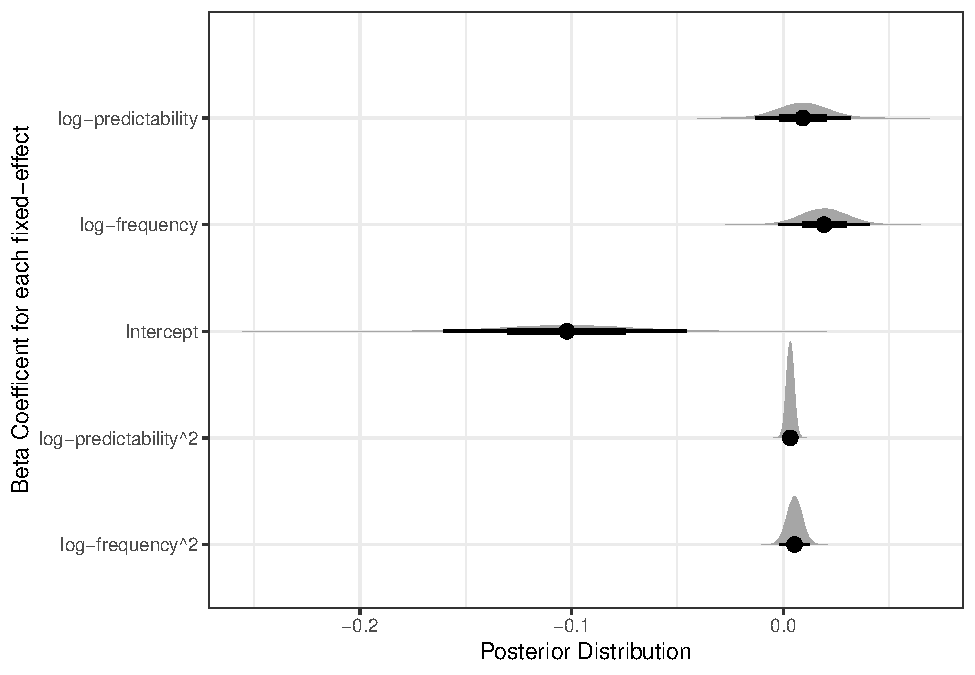
\includegraphics[width=0.8\linewidth]{write-up_files/figure-latex/posteriorplotFullQuadratic-1} 

}

\caption{Plot of the posterior distribution for the beta value of each fixed-effect in our Bayesian quadratic regression model. The y axis contains the different fixed-effects and the x-axis contains the posterior distribution of beta values for the corresponding fixed-effect.}\label{fig:posteriorplotFullQuadratic}
\end{figure}



\begin{figure}

{\centering 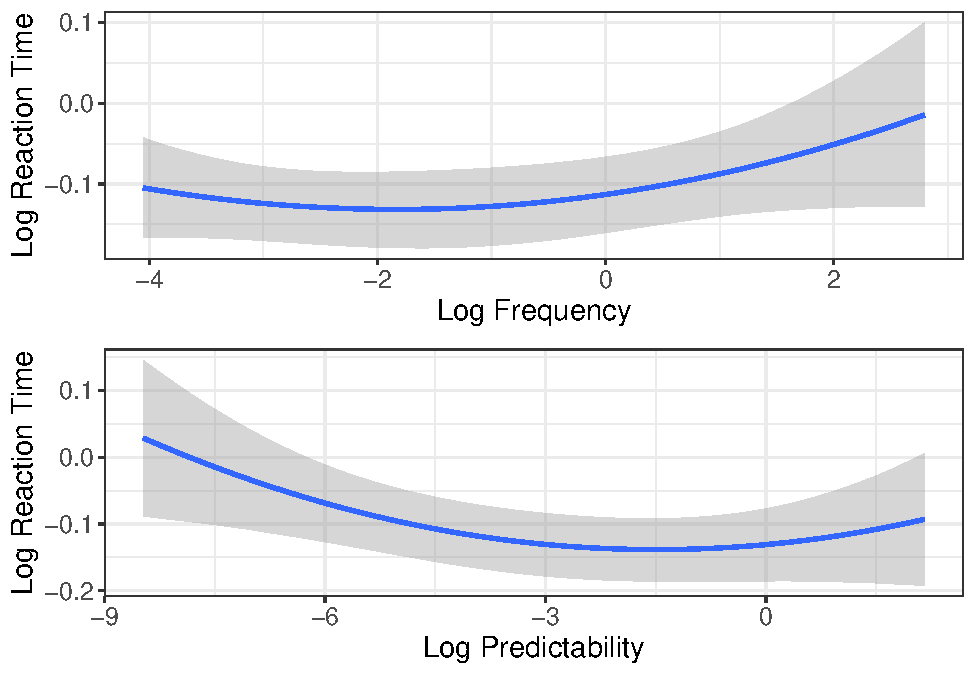
\includegraphics[width=0.8\linewidth]{write-up_files/figure-latex/FullQuadraticPlot-1} 

}

\caption{Visualization of the model results from Table \ref{tab:gamModelTab} for frequency (top) and predictability (bottom). Frequencies are per million.}\label{fig:FullQuadraticPlot}
\end{figure}

Finally tables \ref{tab:brmsFreq} and \ref{tab:brmsPredic} present the results for the quadratic regression models including only frequency and \(frequency^2\) as well as the quadratic regression model including only predictability and \(predictability^2\) respectively:



\begin{table}[H]

\begin{center}
\begin{threeparttable}

\caption{\label{tab:brmsFreq}Results for the Bayesian quadratic regression model containing only frequency and \(frequency^2\).}

\begin{tabular}{lllll}
\toprule
 & \multicolumn{1}{c}{Estimate} & \multicolumn{1}{c}{Est.Error} & \multicolumn{1}{c}{Q2.5} & \multicolumn{1}{c}{Q97.5}\\
\midrule
Intercept & -0.10 & 0.02 & -0.15 & -0.05\\
log-frequency & 0.02 & 0.01 & 0.00 & 0.04\\
Duration & -0.08 & 0.10 & -0.28 & 0.11\\
log-frequency\textasciicircum{}2 & 0.01 & 0.00 & 0.00 & 0.01\\
\bottomrule
\end{tabular}

\end{threeparttable}
\end{center}

\end{table}



\begin{table}[H]

\begin{center}
\begin{threeparttable}

\caption{\label{tab:brmsPredic}Results for the Bayesian quadratic regression model containing only predidctability and \(predictability^2\).}

\begin{tabular}{lllll}
\toprule
 & \multicolumn{1}{c}{Estimate} & \multicolumn{1}{c}{Est.Error} & \multicolumn{1}{c}{Q2.5} & \multicolumn{1}{c}{Q97.5}\\
\midrule
Intercept & -0.10 & 0.02 & -0.15 & -0.05\\
log-predictability & 0.02 & 0.01 & 0.00 & 0.04\\
Duration & -0.08 & 0.10 & -0.28 & 0.11\\
log-predictability\textasciicircum{}2 & 0.01 & 0.00 & 0.00 & 0.01\\
\bottomrule
\end{tabular}

\end{threeparttable}
\end{center}

\end{table}

While the confidence interval for the quadratic term in both models crosses zero, over 95\% of the posterior samples for \(log-frequency^2\) were greater than zero and over 96 percent of the posterior samples for \(log-predictability^2\) were greater than zero. A visualization of the posterior distributions for both models are presented in Figure \ref{fig:FreqOnlyBetaPlot} and Figure \ref{fig:PredicOnlyBetaPlot}. Further, visualizations of the model predictions are also included below in Figures \ref{fig:FreqOnlyPlot} and \ref{fig:PredicOnlyPlot}.

\begin{figure}

{\centering 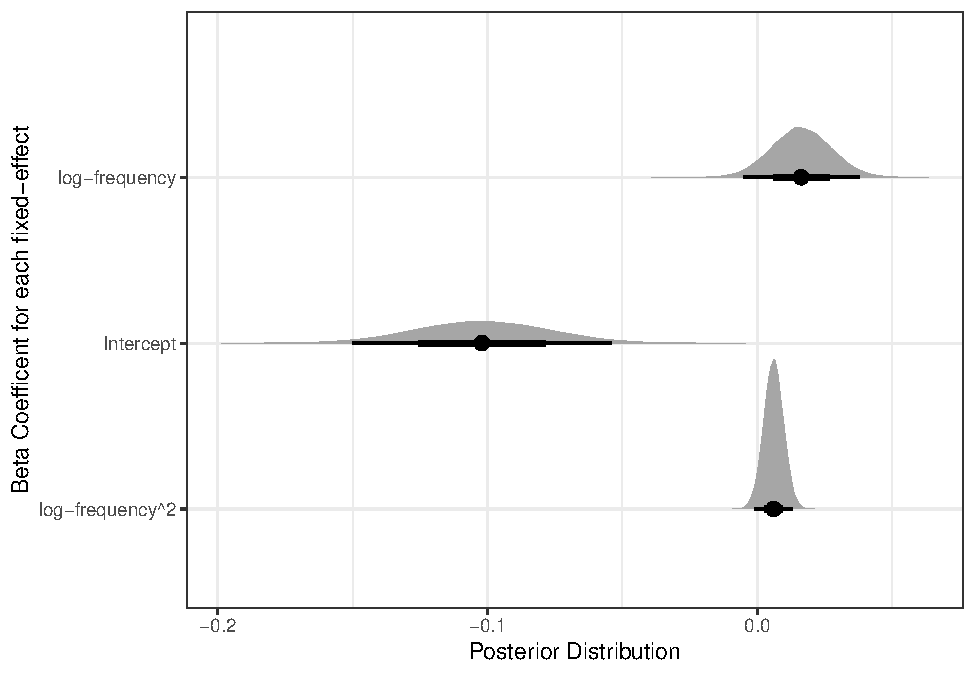
\includegraphics[width=0.8\linewidth]{write-up_files/figure-latex/FreqOnlyBetaPlot-1} 

}

\caption{Plot of the posterior distribution for the beta value of each fixed-effect in our frequency-only quadratic regression model. The y axis contains the different fixed-effects and the x-axis contains the posterior distribution of beta values for the corresponding fixed-effect.}\label{fig:FreqOnlyBetaPlot}
\end{figure}

\begin{figure}

{\centering 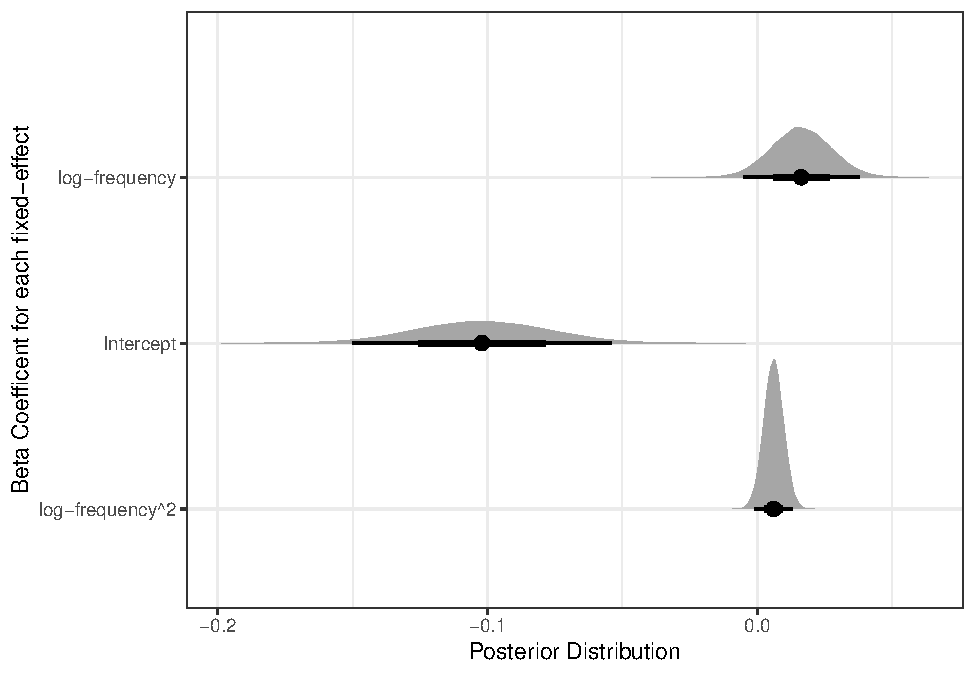
\includegraphics[width=0.8\linewidth]{write-up_files/figure-latex/PredicOnlyBetaPlot-1} 

}

\caption{Plot of the posterior distribution for the beta value of each fixed-effect in our predictability-only quadratic regression model. The y axis contains the different fixed-effects and the x-axis contains the posterior distribution of beta values for the corresponding fixed-effect.}\label{fig:PredicOnlyBetaPlot}
\end{figure}

\begin{figure}

{\centering 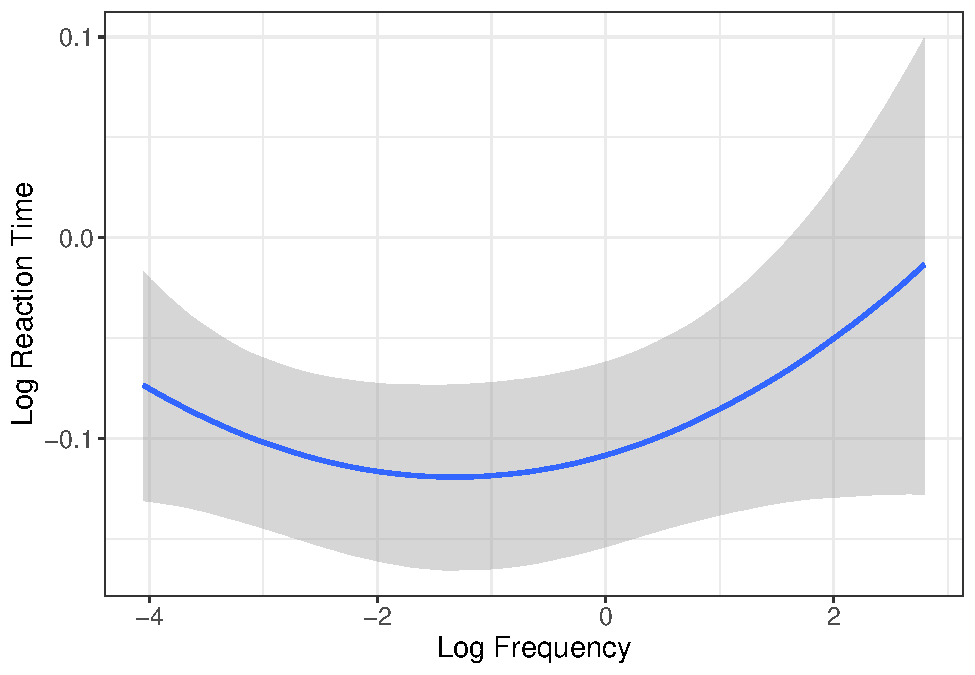
\includegraphics[width=0.6\linewidth]{write-up_files/figure-latex/FreqOnlyPlot-1} 

}

\caption{Model predictions for the effects of frequency on reaction times for the frequency-only Bayesian quadratic model.}\label{fig:FreqOnlyPlot}
\end{figure}

\begin{figure}

{\centering 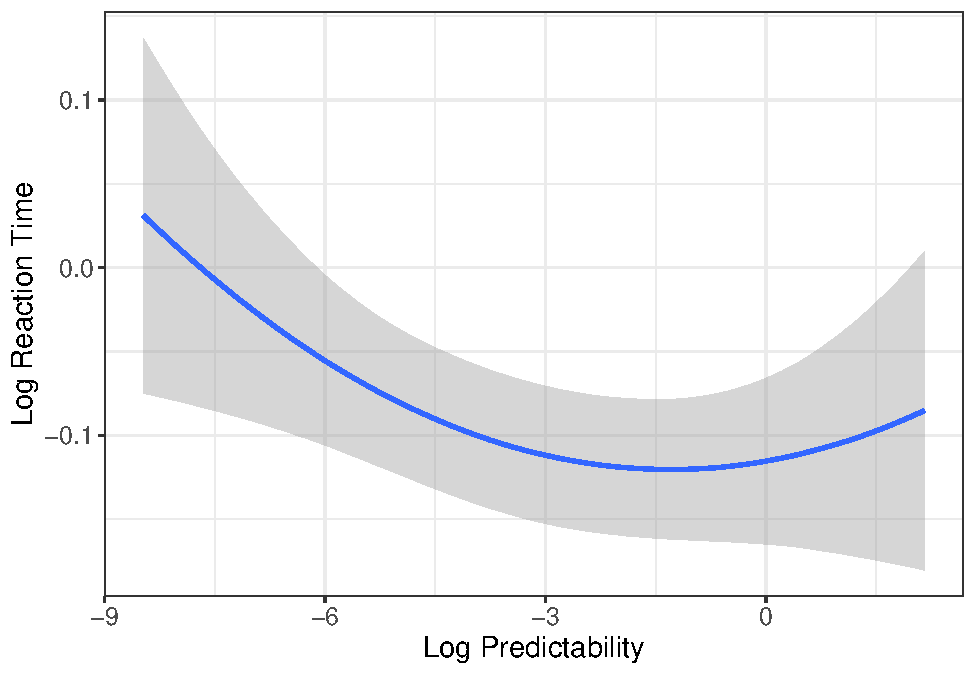
\includegraphics[width=0.6\linewidth]{write-up_files/figure-latex/PredicOnlyPlot-1} 

}

\caption{Model predictions for the effect of predictability on reaction times for the predictability-only models.}\label{fig:PredicOnlyPlot}
\end{figure}

\hypertarget{discussion}{%
\section{Discussion}\label{discussion}}

The present study examined the effects of frequency and predictability on the recognizability of the particle up in English phrasal verbs. We find a u-shaped effect for both frequency and predictability on recognizability. These results suggest that the most predictable and/or highest frequency items have a lack of internal structure relative to their lower frequency/predictability counterparts. We also find no significant differences between phrasal verbs (e.g., \emph{pick up}) and non-phrasal verbs (e.g., \emph{walk up}), suggesting that this effect is driven primarily by the statistical distribution of the input as opposed to semantic or syntactic properties. Although future research would do well to examine whether semantic properties (such as the extent to which a phrase is semantically transparent) mediate this effect.

First, our results suggest that both frequency and predictability drive storage, as we see the increased recognition times for both high frequency and high predictability items. Though it is possible that the statistics driving the increased recognition times are different from those that drive storage, as we will discuss further below.

Our results also show that as frequency or predictability increases, recognition time decreases until reaching the highest frequency/predictability items where there is an increase in recognition time. These findings demonstrate competition between different levels (e.g., competition between a holistically stored phrase and its individual words) during processing. That is, they suggest that during processing, holistically stored items compete with their parts for recognition. These results replicate similar findings (Healy, 1976; e.g., Kapatsinski \& Radicke, 2009; Minkoff \& Raney, 2000). For example, as stated earlier, Healy (1976) found that people make more letter-detection errors in high-frequency words (e.g., \emph{the}) than in lower frequency words. Further, Minkoff and Raney (2000) found that letters are more difficult to detect in high-frequency nouns than in low-frequency nouns. These results suggest that recognizing words (and by extension, holistically stored phrases) does not necessarily require recognizing the individual letters or sounds that comprise them.

One possible explanation for this competition is that the increase in recognition time reflects a loss of internal structure for the items that show said increase. That is, it is possible that over time, more experience with the items results in a loss of the internal structure, or a weakening of the associations between the individual words and the meaning of the phrase (as demonstrated in Figure \ref{fig:lossInternal})

Another possible account is that perhaps the internal structure was never learned to begin with. For example, children are experts at statistical learning and use transitional probabilities to divide the continuous speech stream (Saffran et al., 1996). High predictability phrases, by definition, have higher transitional probabilities between words. Thus if children are relying on transitional probabilities to separate speech into individual words, the most predictable phrases may not be separated out of the speech stream initially. Though this explanation doesn't necessarily explain the frequency effect.

Further, many high-frequency (e.g., \emph{set up}) and high-predictability (e.g., \emph{conjure up}) phrases have semantically vague relationships that might make it difficult to split them up on a semantic basis. It seems plausible then that maybe these phrases weren't learned as individual words initially and thus the internal structure for the holistically stored item may not have been learned.

If it is the case that the internal structure for the phrase was never learned, it would explain nicely why we see an increase in recognition times for \emph{up}: as one encounters the phrase more often, this could weaken the association between the individual words and the holistically stored phrase (which lacks internal structure). Indeed, this parallels findings from the learning literature where an association between two cues and an outcome can cause the association between the individual cues and that outcome to weaken {[}i.e., an overexpectation effect; for example, when a noise and light are paired with a shock, the strength of the association between the individual cues and the shock decreases, Bouton (2007){]}. In this case, the two cues would be the words (e.g., \emph{pick} and \emph{up}) and the outcome would be the holistically stored meaning (e.g., \emph{pick up}).

It also mirrors evidence from the artificial language learning literature, where it's been demonstrated that increased exposure to a morpheme or word makes one more confident that the meaning of that morpheme or word is not used to express other meanings (Harmon \& Kapatsinski, 2017; Xu \& Tenenbaum, 2007). For example, Harmon and Kapatsinski (2017) demonstrated that increased exposure to a novel suffix makes learners less likely to extend it to novel meanings in comprehension. While the meanings in our case are the same, the representations are different (compositional vs holistic representation). It is possible that increased exposure to \emph{pick up}, for example, entrenches the association between the form \emph{pick up} and the holistically stored representation, inhibiting the association between the form and the compositional representation. This would explain why for the highest frequency and predictability items recognition time increases: accessing the holistically stored phrase inhibits access of the compositional form, making it harder to recognize the individual parts (though perhaps inhibition is not even necessary to account for the increase in reaction time).

Further, if the lack of internal representation is a function of our learning mechanisms, it may not be surprising that both predictability and frequency drive this lack of representation, since our brain employs both Hebbian (frequency-driven learning) and error-driven learning mechanisms {[}predictability-driven learning; Kapatsinski (2018); Ashby, Ennis, and Spiering (2007){]}.

Our results also open an interesting question of how gradient the internal structure is. For example, our results suggest that the internal structure isn't completely eroded even for the highest frequency/most predictable items, since participants are clearly aware that the segment up is contained in the phrase, it just takes them longer to recognize. On the other hand, the internal structure seems to have degraded at least a little bit, since participants are not as quick to recognize the segment as we would expect. One possibility is that the internal structure is much more gradient. That is, it is possible that part of the internal representation has weakened.

Alternatively, it's possible that the internal structure for the holistic item is completely eroded and what we see is actually a recognition of \emph{up} driven by the compositional interpretation. That is, it is possible that the holistically stored phrase (e.g., \emph{pick up}) has completely lost the internal representation of up. However, that doesn't mean participants are unable to also decode the meaning by combining \emph{pick} with \emph{up}. The delayed recognition times could be reflecting the composition time. If this is the case, it opens up the question of whether experience with a phrase increases the strength of the association between the words and the representation of the phrase, or the strength of the association between the words and the representation of each individual words, or both.

Finally it is possible that our results may not reflect a lack of internal representation but instead reflect a processing strategy. For example, it is possible that since high-frequency and high-predictability items are accessed faster, participants may move on from processing the form of the phrase once they've accessed the meaning. Indeed, this argument has been put forth by (Healy, 1994; and echoed by Kapatsinski \& Radicke, 2009) who argued that once the larger unit is recognized, recognition of the internal parts is terminated and processing moves on. Although it's worth pointing out that this necessitates a representation without internal structure, since it's unclear how else one can access a phrase or a word without accessing its parts.

In summary, we demonstrate that both frequency and predictability seem to drive the holistic storage of phrasal verbs, and these holistically stored items compete with their component parts during lexical access. Our paper also leaves many open questions about whether holistically stored items have no internal structure from the onset due to learning mechanisms, or if this is lost over time as a function of experience. Further, we leave open the question of whether internal structure is gradient or an all-or-nothing representation.

\newpage

\hypertarget{references}{%
\section{References}\label{references}}

\hypertarget{refs}{}
\begin{CSLReferences}{1}{0}
\leavevmode\vadjust pre{\hypertarget{ref-arnon2010}{}}%
Arnon, I., \& Snider, N. (2010). More than words: Frequency effects for multi-word phrases. \emph{Journal of Memory and Language}, \emph{62}(1), 67--82. \url{https://doi.org/10.1016/j.jml.2009.09.005}

\leavevmode\vadjust pre{\hypertarget{ref-ashbyNeurobiologicalTheoryAutomaticity2007}{}}%
Ashby, F. G., Ennis, J. M., \& Spiering, B. J. (2007). A neurobiological theory of automaticity in perceptual categorization. \emph{Psychological Review}, \emph{114}(3), 632. Retrieved from \url{https://psycnet.apa.org/journals/rev/114/3/632/}

\leavevmode\vadjust pre{\hypertarget{ref-boutonLearning2007}{}}%
Bouton, M. E. (2007). \emph{Learning and behavior: A contemporary synthesis.} Sinauer Associates. Retrieved from \url{https://psycnet.apa.org/record/2006-21409-000}

\leavevmode\vadjust pre{\hypertarget{ref-brms}{}}%
Bürkner, P.-C. (2017). {brms}: An {R} package for {Bayesian} multilevel models using {Stan}. \emph{Journal of Statistical Software}, \emph{80}(1), 1--28. \url{https://doi.org/10.18637/jss.v080.i01}

\leavevmode\vadjust pre{\hypertarget{ref-bybee2002}{}}%
Bybee, J. (2002). Word frequency and context of use in the lexical diffusion of phonetically conditioned sound change. \emph{Language Variation and Change}, \emph{14}(3), 261--290. \url{https://doi.org/10.1017/S0954394502143018}

\leavevmode\vadjust pre{\hypertarget{ref-bybee2003}{}}%
Bybee, J. (2003). \emph{Phonology and language use} (Vol. 94). Cambridge University Press.

\leavevmode\vadjust pre{\hypertarget{ref-bybee2001}{}}%
Bybee, J., \& Hopper, P. (2001). Introduction to frequency and the emergence of linguistic structure. \emph{Typological Studies in Language}, \emph{45}, 126.

\leavevmode\vadjust pre{\hypertarget{ref-bybee1999}{}}%
Bybee, J., \& Scheibman, J. (1999). The effect of usage on degrees of constituency: The reduction of don't in english. \emph{Linguistics}, \emph{37}(4). \url{https://doi.org/10.1515/ling.37.4.575}

\leavevmode\vadjust pre{\hypertarget{ref-christiansen2017}{}}%
Christiansen, M. H., \& Arnon, I. (2017). More than words: The role of multiword sequences in language learning and use. \emph{Topics in Cognitive Science}, \emph{9}(3), 542--551. \url{https://doi.org/10.1111/tops.12274}

\leavevmode\vadjust pre{\hypertarget{ref-goldberg2003}{}}%
Goldberg, A. E. (2003). Constructions: A new theoretical approach to language. \emph{Trends in Cognitive Sciences}, \emph{7}(5), 219--224. \url{https://doi.org/10.1016/S1364-6613(03)00080-9}

\leavevmode\vadjust pre{\hypertarget{ref-harmonPuttingOldTools2017}{}}%
Harmon, Z., \& Kapatsinski, V. (2017). Putting old tools to novel uses: The role of form accessibility in semantic extension. \emph{Cognitive Psychology}, \emph{98}, 22--44. \url{https://doi.org/10.1016/j.cogpsych.2017.08.002}

\leavevmode\vadjust pre{\hypertarget{ref-hay2001}{}}%
Hay, J. (2001). Lexical frequency in morphology: Is everything relative? \emph{Linguistics}, \emph{39}(376), 1041--1070. \url{https://doi.org/10.1515/ling.2001.041}

\leavevmode\vadjust pre{\hypertarget{ref-healy1976}{}}%
Healy, A. F. (1976). Detection errors on the word the: Evidence for reading units larger than letters. \emph{Journal of Experimental Psychology: Human Perception and Performance}, \emph{2}(2), 235. Retrieved from \url{https://psycnet.apa.org/journals/xhp/2/2/235/}

\leavevmode\vadjust pre{\hypertarget{ref-healy1994}{}}%
Healy, A. F. (1994). Letter detection: A window to unitization and other cognitive processes in reading text. \emph{Psychonomic Bulletin \& Review}, \emph{1}(3), 333--344. \url{https://doi.org/10.3758/BF03213975}

\leavevmode\vadjust pre{\hypertarget{ref-hochreiterLSTM1997}{}}%
Hochreiter, S., \& Schmidhuber, J. (1997). Long short-term memory. \emph{Neural Computation}, \emph{9}(8), 17351780. Retrieved from \url{https://ieeexplore.ieee.org/abstract/document/6795963/}

\leavevmode\vadjust pre{\hypertarget{ref-hooper1976}{}}%
Hooper, J. B. (1976). Word frequency in lexical diffusion and the source of morphophonological change. \emph{Current Progress in Historical Linguistics}, \emph{96}, 105.

\leavevmode\vadjust pre{\hypertarget{ref-houghtonTaskdependentConsequencesDisfluency2023}{}}%
Houghton, Z., Kato, M., Baese-Berk, M., \& Vaughn, C. (2023). Task-dependent consequences of disfluency in perception of native and non-native speech. \emph{Applied Psycholinguistics}, 1--17. \url{https://doi.org/10.1017/S0142716423000486}

\leavevmode\vadjust pre{\hypertarget{ref-kapatsinski2018}{}}%
Kapatsinski, V. (2018). \emph{Changing minds changing tools: From learning theory to language acquisition to language change}. MIT Press.

\leavevmode\vadjust pre{\hypertarget{ref-kapatsinskiHierarchicalInferenceSound2021}{}}%
Kapatsinski, V. (2021). Hierarchical inference in sound change: Words, sounds, and frequency of use. \emph{Frontiers in Psychology}, \emph{12}(August). \url{https://doi.org/10.3389/fpsyg.2021.652664}

\leavevmode\vadjust pre{\hypertarget{ref-kapatsinski2009}{}}%
Kapatsinski, V., \& Radicke, J. (2009). \emph{Frequency and the emergence of prefabs: Evidence from monitoring}. (January 2009), 499. \url{https://doi.org/10.1075/tsl.83.14kap}

\leavevmode\vadjust pre{\hypertarget{ref-lee2015}{}}%
Lee, O., \& Kapatsinski, V. (2015). \emph{Frequency effects in morphologisation of korean /n/-epenthesis}. 1--23.

\leavevmode\vadjust pre{\hypertarget{ref-levyProcessingExtraposedStructures2012}{}}%
Levy, R., Fedorenko, E., Breen, M., \& Gibson, E. (2012). The processing of extraposed structures in english. \emph{Cognition}, \emph{122}(1), 12--36. \url{https://doi.org/10.1016/j.cognition.2011.07.012}

\leavevmode\vadjust pre{\hypertarget{ref-maye2000}{}}%
Maye, J., \& Gerken, L. (2000). \emph{Learning phonemes without minimal pairs}. \emph{2}, 522533.

\leavevmode\vadjust pre{\hypertarget{ref-minkoff2000}{}}%
Minkoff, S. R. B., \& Raney, G. E. (2000). Letter-Detection Errors in the Word The: Word Frequency Versus Syntactic Structure. \emph{Scientific Studies of Reading}, \emph{4}(1), 55--76. \url{https://doi.org/10.1207/S1532799XSSR0401_5}

\leavevmode\vadjust pre{\hypertarget{ref-mollica2019}{}}%
Mollica, F., \& Piantadosi, S. T. (2019). Humans store about 1.5 megabytes of information during language acquisition. \emph{Royal Society Open Science}, \emph{6}(3), 181393. \url{https://doi.org/10.1098/rsos.181393}

\leavevmode\vadjust pre{\hypertarget{ref-morgan2016}{}}%
Morgan, E., \& Levy, R. (2016). Frequency-dependent regularization in iterated learning. \emph{The Evolution of Language: Proceedings of the 11th International Conference (EVOLANGX11)}, (2015).

\leavevmode\vadjust pre{\hypertarget{ref-nooteboom2002}{}}%
Nooteboom, S., Nooteboom, S., Weerman, F., \& Wijnen, F. (2002). \emph{Storage and computation in the language faculty}. Springer Science \& Business Media.

\leavevmode\vadjust pre{\hypertarget{ref-olejarczuk2018}{}}%
Olejarczuk, P., Kapatsinski, V., \& Baayen, R. H. (2018). Distributional learning is error-driven: The role of surprise in the acquisition of phonetic categories. \emph{Linguistics Vanguard}, \emph{4}(s2), 1--9. \url{https://doi.org/10.1515/lingvan-2017-0020}

\leavevmode\vadjust pre{\hypertarget{ref-Rpackage}{}}%
R Core Team. (2023). \emph{R: A language and environment for statistical computing}. Vienna, Austria: R Foundation for Statistical Computing. Retrieved from \url{https://www.R-project.org/}

\leavevmode\vadjust pre{\hypertarget{ref-ramscar2013}{}}%
Ramscar, M., Dye, M., \& Klein, J. (2013). Children value informativity over logic in word learning. \emph{Psychological Science}, \emph{24}(6), 1017--1023. \url{https://doi.org/10.1177/0956797612460691}

\leavevmode\vadjust pre{\hypertarget{ref-saffran1996}{}}%
Saffran, J. R., Aslin, R. N., \& Newport, E. L. (1996). Statistical Learning by 8-Month-Old Infants. \emph{Science}, \emph{274}(5294), 1926--1928. \url{https://doi.org/10.1126/science.274.5294.1926}

\leavevmode\vadjust pre{\hypertarget{ref-siegelman2015}{}}%
Siegelman, N., \& Arnon, I. (2015). The advantage of starting big: Learning from unsegmented input facilitates mastery of grammatical gender in an artificial language. \emph{Journal of Memory and Language}, \emph{85}, 60--75. \url{https://doi.org/10.1016/j.jml.2015.07.003}

\leavevmode\vadjust pre{\hypertarget{ref-siyanova-chanturia2011}{}}%
Siyanova-Chanturia, A., Conklin, K., \& Heuven, W. J. B. van. (2011). Seeing a phrase {``}time and again{"} matters: The role of phrasal frequency in the processing of multiword sequences. \emph{Journal of Experimental Psychology: Learning Memory and Cognition}, \emph{37}(3), 776--784. \url{https://doi.org/10.1037/a0022531}

\leavevmode\vadjust pre{\hypertarget{ref-stemberger1986}{}}%
Stemberger, J. P., \& MacWhinney, B. (1986). Frequency and the lexical storage of regularly inflected forms. \emph{Memory \& Cognition}, \emph{14}(1), 17--26. \url{https://doi.org/10.3758/BF03209225}

\leavevmode\vadjust pre{\hypertarget{ref-stemberger2004}{}}%
Stemberger, J. P., \& MacWhinney, B. (2004). Are inflected forms stored in the lexicon. \emph{Morphology: Critical Concepts in Linguistics}, \emph{6}, 107122.

\leavevmode\vadjust pre{\hypertarget{ref-tomasello2005}{}}%
Tomasello, M. (2005). \emph{Constructing a language: A usage-based theory of language acquisition}. Harvard university press.

\leavevmode\vadjust pre{\hypertarget{ref-vaswaniAttentionAllYou2017}{}}%
Vaswani, A., Shazeer, N., Parmar, N., Uszkoreit, J., Jones, L., Gomez, A. N., \ldots{} Polosukhin, I. (2017). Attention is all you need. \emph{Advances in Neural Information Processing Systems}, \emph{30}. Retrieved from \url{https://proceedings.neurips.cc/paper/7181-attention-is-all}

\leavevmode\vadjust pre{\hypertarget{ref-wang2003}{}}%
Wang, Y., Liu, D., \& Wang, Y. (2003). Discovering the Capacity of Human Memory. \emph{Brain and Mind}, \emph{4}(2), 189--198. \url{https://doi.org/10.1023/A:1025405628479}

\leavevmode\vadjust pre{\hypertarget{ref-mgcv}{}}%
Wood, S. N. (2011). \emph{Fast stable restricted maximum likelihood and marginal likelihood estimation of semiparametric generalized linear models}. \emph{73}, 3--36.

\leavevmode\vadjust pre{\hypertarget{ref-xuWordLearningBayesian2007}{}}%
Xu, F., \& Tenenbaum, J. B. (2007). Word learning as bayesian inference. \emph{Psychological Review}, \emph{114}(2), 245. Retrieved from \url{https://psycnet.apa.org/record/2007-05396-002}

\leavevmode\vadjust pre{\hypertarget{ref-yi2002}{}}%
Yi, B.-W. (2002). Ŭmun hyŏnsanggwa pindo hyogwa {[}the effects of frequency and phonology{]}. \emph{Han'gugŏhak}, \emph{15}, 161--183.

\leavevmode\vadjust pre{\hypertarget{ref-zwitserlood2018}{}}%
Zwitserlood, P. (2018). Processing and representation of morphological complexity in native language comprehension and production. \emph{The Construction of Words: Advances in Construction Morphology}, 583--602. \url{https://doi.org/10.1007/978-3-319-74394-3_20}

\end{CSLReferences}


\end{document}
